% titlepage-demo.tex
\documentclass{beamer}
\usetheme{Boadilla}
\usepackage{multirow}
\usepackage[absolute,overlay]{textpos} 
\newenvironment{reference}[2]{% 
  \begin{textblock*}{\textwidth}(#1,#2) 
      \footnotesize\it\bgroup\color{red!50!black}}{\egroup\end{textblock*}} 



\begin{document}


\begin{frame}[t]{Big Picture}
\begin{center}
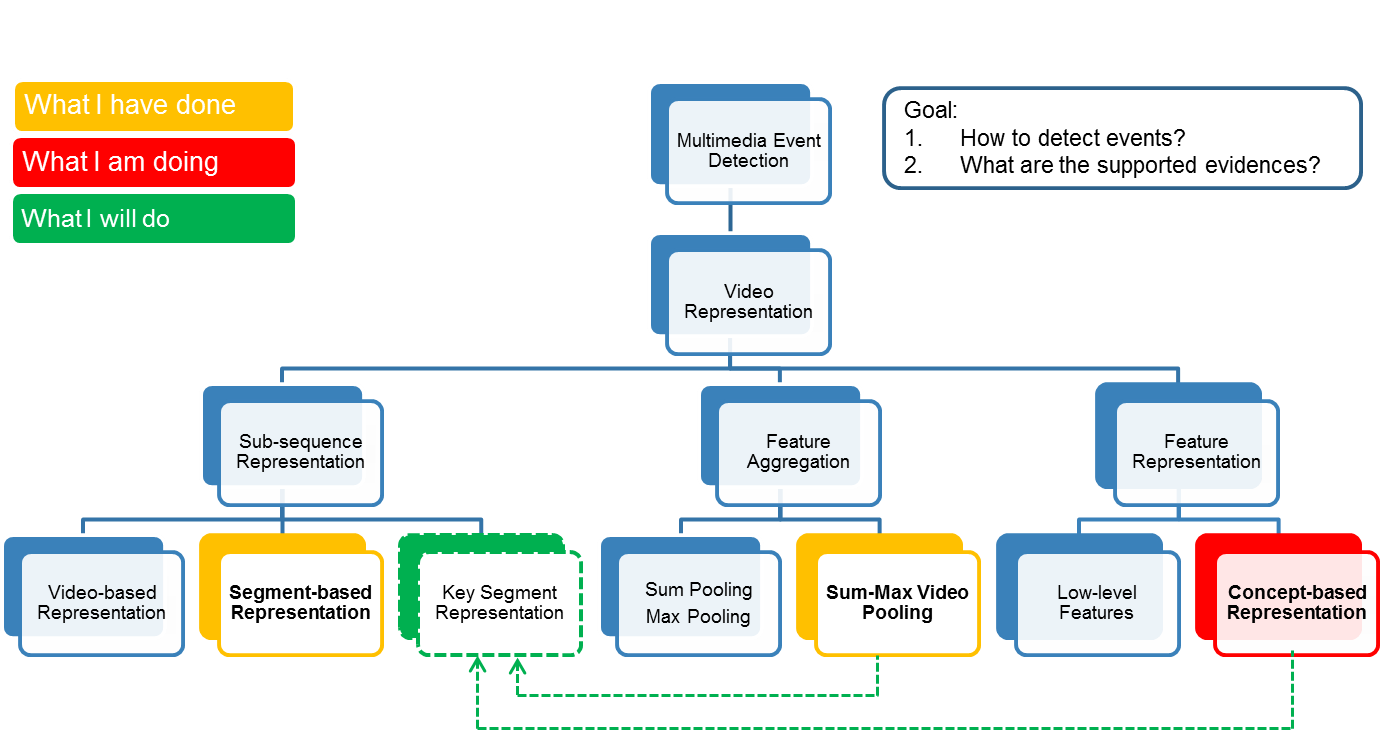
\includegraphics[width=12cm,height=7cm]{images/bigpicture.png}
\end{center}

\end{frame}

% % part 1
\begin{frame}[t]{Challenges of Multimedia Event Detection}
\begin{center}
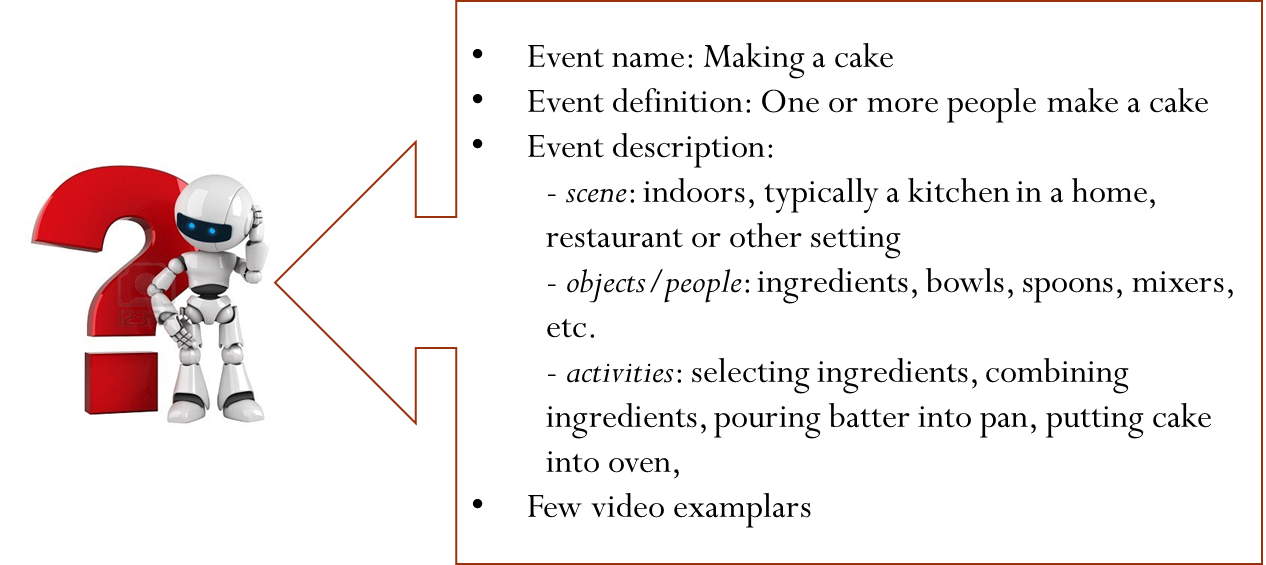
\includegraphics[width=10cm,height=4.5cm]{images/challenge3.png}
\end{center}

\begin{itemize}
\item Searching for ad hoc events 
\begin{itemize}
\item Limited number of video examples
\item Textual descriptions are readily understood by humans, difficult to encode for machine learning approaches
\end{itemize}

\end{itemize}

\end{frame}


%--- the presentation begins here ----------------%
\begin{frame}[t]{Challenges of Multimedia Event Detection}
\begin{center}
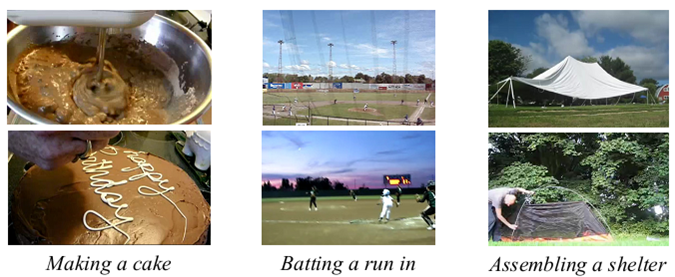
\includegraphics[width=10cm,height=4.5cm]{images/challenge1.png}
\end{center}

\begin{itemize}
\item Large content variation

\begin{itemize}
\item Large number of events
\item Large number of background videos.
\end{itemize}

\end{itemize}

\end{frame}

\begin{frame}[t]{Challenges of Multimedia Event Detection}
\begin{center}
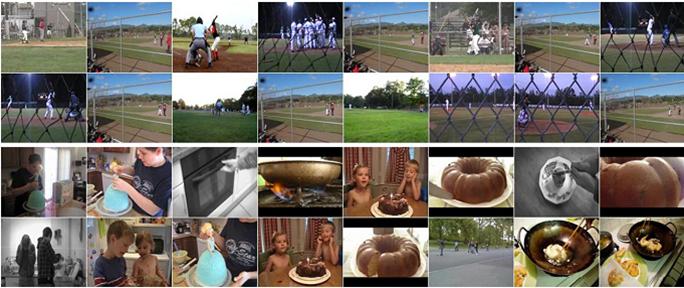
\includegraphics[width=10cm,height=4.5cm]{images/challenge2.png}
\end{center}

\begin{itemize}
\item Uncontrolled capturing conditions 
\begin{itemize}
\item Different time, location,
\item Clutter in the environment, camera motion, etc.
\end{itemize}

\end{itemize}

\end{frame}

% % part 2

\begin{frame}[t]{Approaches for MED}
\begin{itemize}
\item Best MED'10 system: Columbia University, USA

\begin{itemize}
\item Image features: SIFT [Lowe 2004]
\item Motion features: STIP [Laptev 2004]
\item Audio features: MFCC
\end{itemize}
\item Best MED'11 system: BBN VISER, USA
\begin{itemize}
\item Image features: SIFT, SURF, D-SIFT, CHOG, RGB-SIFT
\item Motion features: STIP, D-STIP
\item Audio features: MFCC, FDLP
\end{itemize}

\item Common Approach: Combining multiple modalities (image, video, audio, etc.)
\begin{itemize}
\item For image features: keyframe-based $\rightarrow$ image classification problems
\item For motion features: video-based approach
\end{itemize}

\end{itemize}
\end{frame}

\begin{frame}[t]{Problem with the Video-based Approach}
\begin{center}
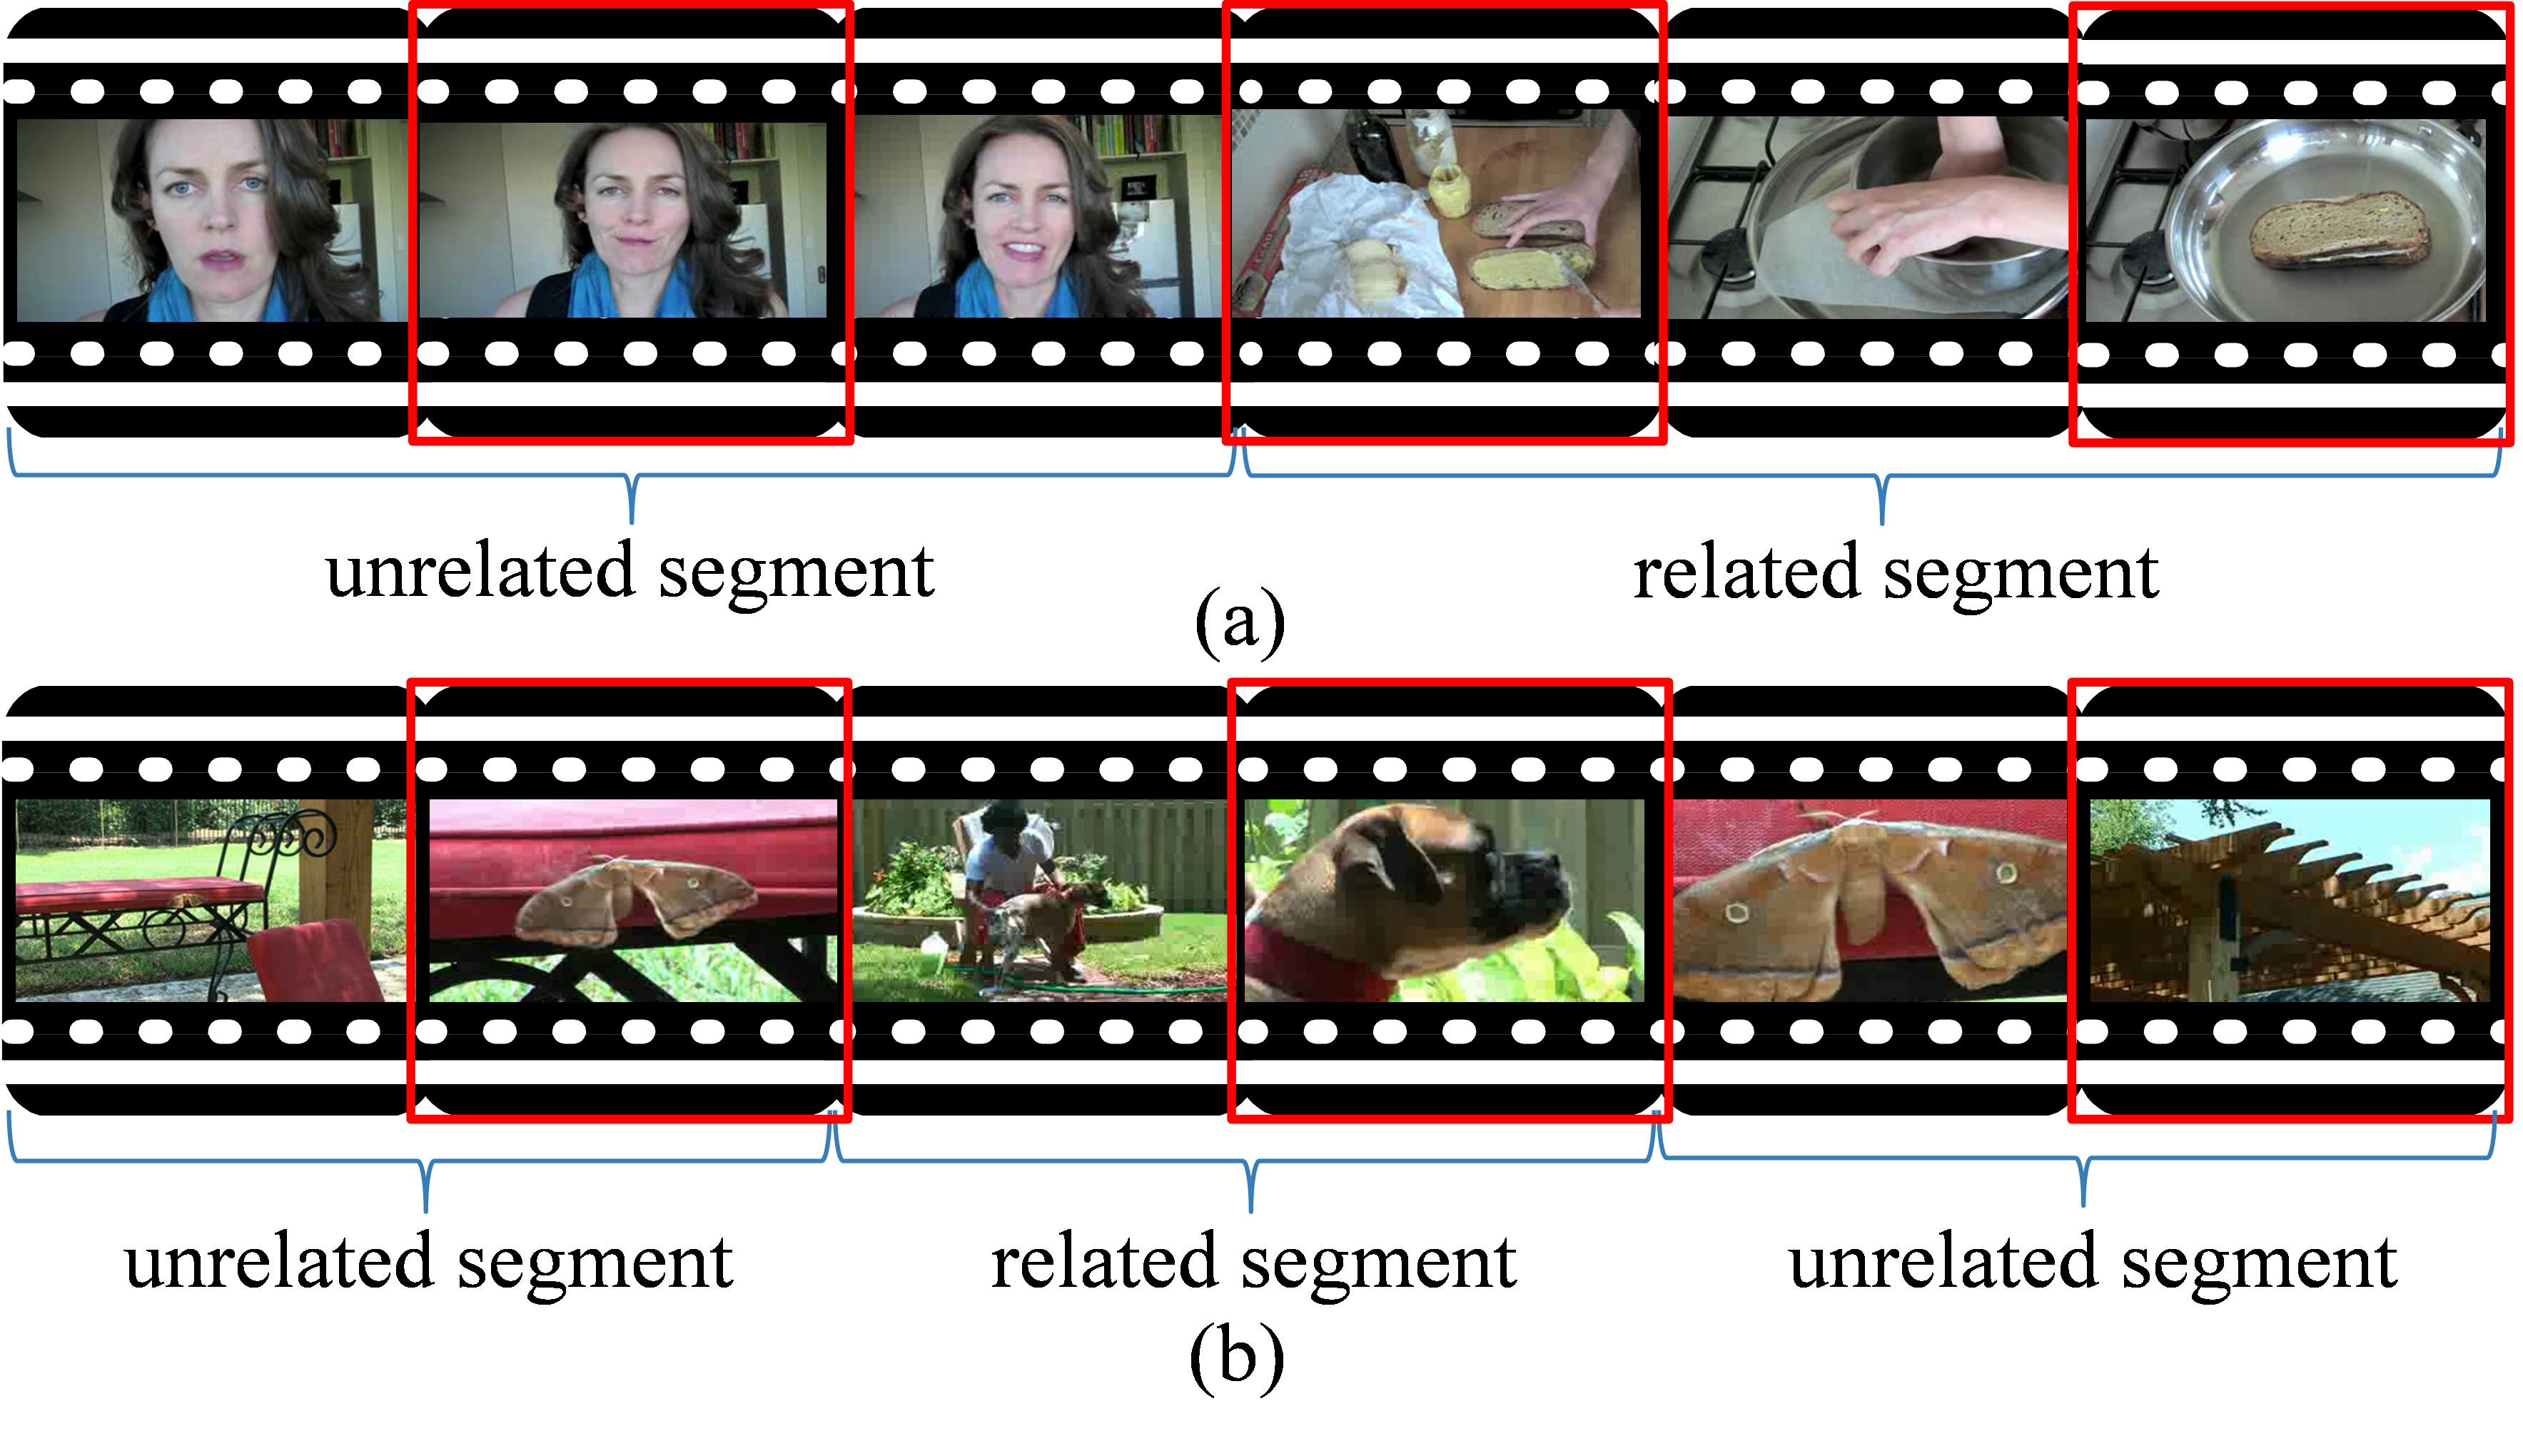
\includegraphics[width=10cm,height=5cm]{images/challenge4.png}
\end{center}

\begin{itemize}
\item MED data is noisy $\rightarrow$ the clues to determine an event may appear within a small segment of the entire video.

\end{itemize}

\end{frame}




\begin{frame}[t]{Our Segment-based Approach}
\begin{center}
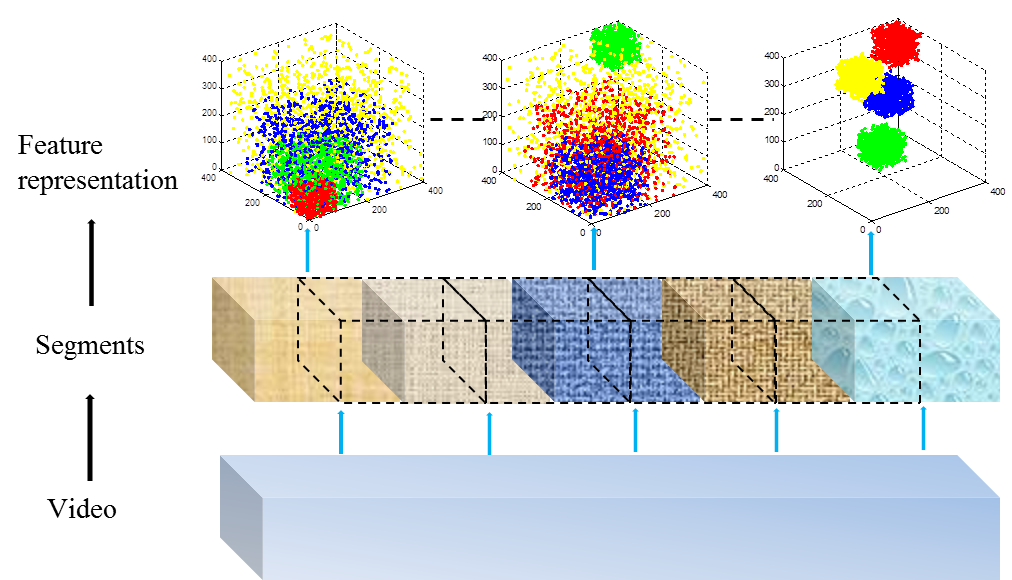
\includegraphics[width=10cm,height=5cm]{images/segment_based.png}
\end{center}

\begin{itemize}
\item The basic idea is to examine shorter segments instead of using the entire video.

\end{itemize}

\end{frame}


\begin{frame}[t]{Comparison}
\begin{table}
\renewcommand{\arraystretch}{1.2}
\caption{Comparison of different segment-based approaches with the video-based approach on the MED 2011 dataset.}
\label{t_med11_comparison}
  \centering
    \scalebox{0.65}{\begin{tabular}{|c|c|c|c|c|c|c|c|}
	\hline
    \multirow{3}[4]{*}{Event/MAP} & \multicolumn{3}{|c|}{Non-overlapping sampling} & \multicolumn{3}{|c|}{Overlapping sampling} & \multirow{3}[4]{*}{Video-based} \\ 
    \cline{2-7}
          & \begin{tabular}[x]{@{}c@{}}Best\\(at 90 s) \end{tabular}
          & \begin{tabular}[x]{@{}c@{}}Late fusion\\(all lengths) \end{tabular}
          & \begin{tabular}[x]{@{}c@{}}Late fusion\\(60, 90, 120 s) \end{tabular}
          & \begin{tabular}[x]{@{}c@{}}Best\\(at 120 s) \end{tabular}
          & \begin{tabular}[x]{@{}c@{}}Late fusion\\(all lengths) \end{tabular}
          & \begin{tabular}[x]{@{}c@{}}Late fusion\\(60, 90, 120 s) \end{tabular} &  \\ \hline
    E006  & \multicolumn{1}{|c|}{\textbf{0.1277}} & 0.1217 & 0.1244 & 0.1151 & 0.1086 & \multicolumn{1}{|c|}{0.1083} & 0.0959 \\ \hline
    
    E007  & \multicolumn{1}{|c|}{0.1521} & 0.1419 & \multicolumn{1}{|c|}{0.1369} & 0.1552 & 0.1610 & \multicolumn{1}{|c|}{\textbf{0.1616}} & 0.1303 \\	\hline
    E008  & \multicolumn{1}{|c|}{0.4923} & \textbf{0.4975} & \multicolumn{1}{|c|}{0.4973} & 0.4969 & 0.4903 & \multicolumn{1}{|c|}{0.4871} & 0.4766 \\	\hline
    E009  & \multicolumn{1}{|c|}{0.2072} & 0.2145 & \multicolumn{1}{|c|}{0.2064} & \textbf{0.2160} & 0.1954 & \multicolumn{1}{|c|}{0.1958} & 0.0943 \\	\hline
    E010  & \multicolumn{1}{|c|}{0.0916} & 0.0771 & \multicolumn{1}{|c|}{0.0753} & 0.1008 & 0.1108 & \multicolumn{1}{|c|}{\textbf{0.1109}} & 0.1020 \\	\hline
    E011  & \multicolumn{1}{|c|}{0.0698} & 0.0805 & \multicolumn{1}{|c|}{0.0813} & \textbf{0.1591} & 0.0819 & \multicolumn{1}{|c|}{0.0845} & 0.0609 \\	\hline
    E012  & \multicolumn{1}{|c|}{\textbf{0.3560}} & 0.3309 & \multicolumn{1}{|c|}{0.3277} & 0.3150 & 0.3293 & \multicolumn{1}{|c|}{0.3341} & 0.2858 \\	\hline
    E013  & \multicolumn{1}{|c|}{0.6030} & 0.6033 & \multicolumn{1}{|c|}{0.6096} & \textbf{0.6188} & 0.5872 & \multicolumn{1}{|c|}{0.5910} & 0.5385 \\	\hline
    E014  & \multicolumn{1}{|c|}{0.2008} & 0.2585 & \multicolumn{1}{|c|}{0.2579} & \textbf{0.2744} & 0.2706 & \multicolumn{1}{|c|}{0.2694} & 0.2138 \\	\hline
    E015  & \multicolumn{1}{|c|}{0.1599} & 0.1583 & \multicolumn{1}{|c|}{0.1622} & 0.1562 & 0.1795 & \multicolumn{1}{|c|}{\textbf{0.1795}} & 0.0964 \\	\hline
    All   & \multicolumn{1}{|c|}{0.2460} & 0.2484 & \multicolumn{1}{|c|}{0.2479} & \textbf{0.2607} & 0.2515 & \multicolumn{1}{|c|}{0.2522} & 0.2095 \\	\hline

    \end{tabular}}%
  \label{tab:addlabel}%
\end{table}%
\end{frame}

% % part 3

\begin{frame}[t]{Problem with the Video-based Approach}
\begin{center}
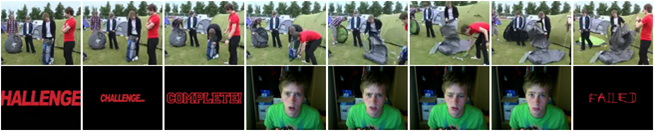
\includegraphics[width=8cm,height=3cm]{images/teaser_image.png}
\end{center}

Example video for "assembling a shelter" event in the TRECVID MED 2010 dataset. The top row shows the relevant frames while the bottom row shows the noisy frames.


$\rightarrow$ Handle in the feature aggregation point of view

\end{frame}

\begin{frame}[t]{Traditional Approach}

\begin{itemize}
\item Building a codebook using K-means, L2 distance, 4000 clusters
\item Assign local descriptors to each cluster based on L2 distance
\item Features that are assigned to a codeword are pooled to get a representative value for that codeword.
\end{itemize}
\begin{center}
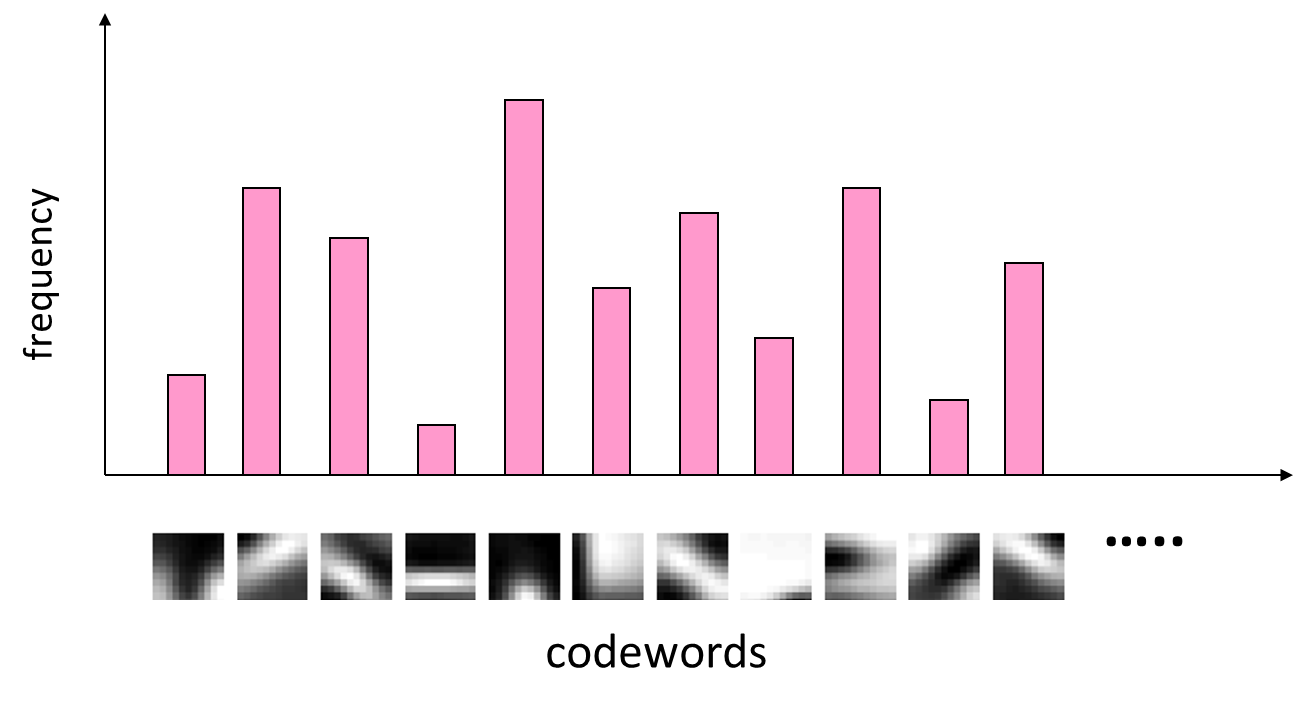
\includegraphics[width=8cm,height=3cm]{images/bow.png}
\end{center}
\begin{itemize}
\item Traditionally, there are two ways:
\begin{itemize}
	\item Sum Pooling: takes a sum over responses to a visual word 
	\item Max Pooling: select the largest value between feature responding to a visual word
\end{itemize}
\end{itemize}

\end{frame}


\begin{frame}[t]{Traditional Approach}

\begin{itemize}
\item Sum pooling and max pooling techniques can be easily adopted for video representation
\item State of art performance with the sum pooling technique in simple video classification/recognition tasks such as sports action videos and studio setting movies
\begin{center}
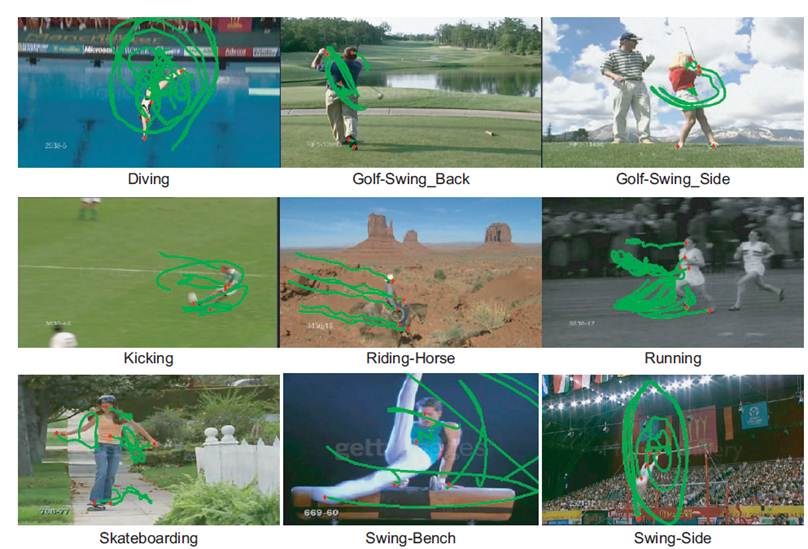
\includegraphics[width=8cm,height=4cm]{images/ucfsports.jpg}
\end{center}
\item However, this observation is not true on complex video datasets where the discriminative features may exist within a small part of the video
\end{itemize}

\end{frame}



\begin{frame}[t]{Sum-max Video Pooling}
Toy example:
\begin{center}
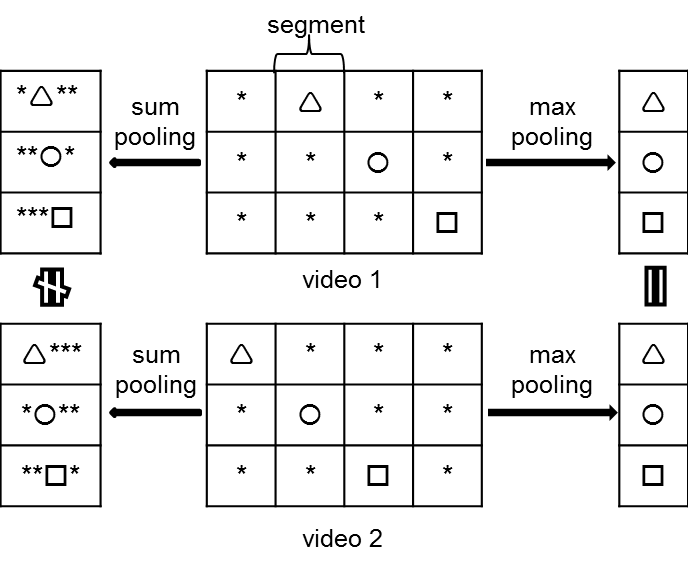
\includegraphics[width=8cm,height=5cm]{images/sum_max.png}
\end{center}
Illustration of sum-max video pooling. $\triangle$, O, $\Box$ represent relevant information; * represents different kinds of irrelevant information, which is popular in complex event data.
\end{frame}

\begin{frame}[t]{Sum-max Video Pooling}
\begin{center}
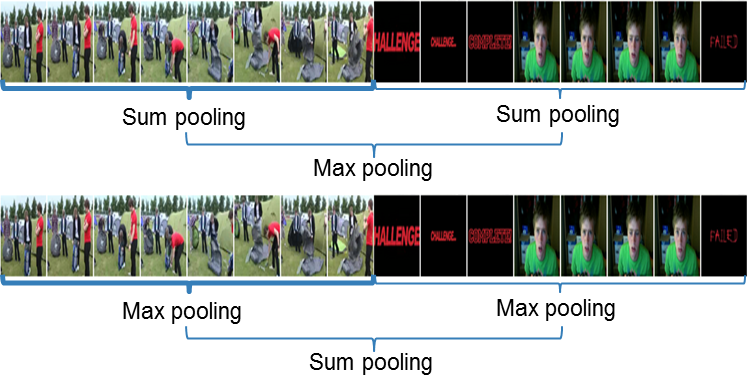
\includegraphics[width=8cm,height=5cm]{images/summax_maxsum.png}
\end{center}
Example of applying sum-max video pooling (top) and max-sum video pooling (bottom) methods on an "assembling a shelter" event video. It can be seen from the top image that after applying max pooling at the segment level, only relevant frames are encoded in the final representation.
\end{frame}


% % part 4

\begin{frame}[t]{Research Questions}

\begin{itemize}
\item Labelled vs. Random Concept Detector?
\item How Many Random Concepts?
\item Influence of Number of Pseudo Positives?
\end{itemize}

\end{frame}


\begin{frame}[t]{Framework}
\begin{center}
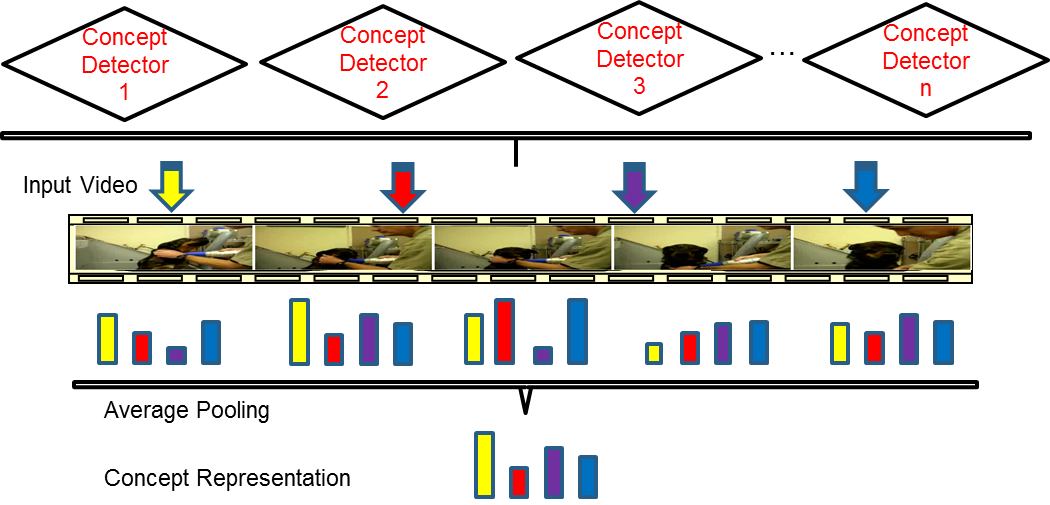
\includegraphics[width=10cm,height=6.5cm]{images/framework_representation.png}
\end{center}

Framework to generate concept-based representation for video.

\end{frame}

\begin{frame}[t]{Labelled vs. Random Concept Detector?}
\begin{center}
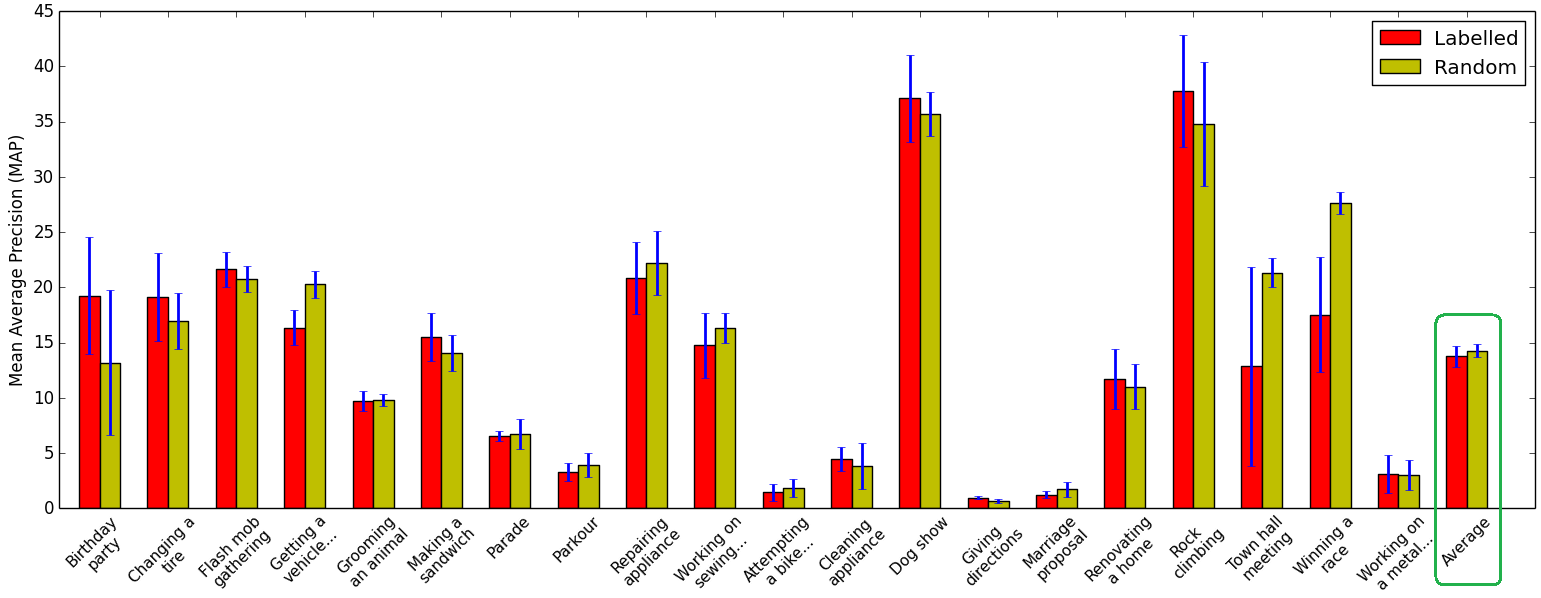
\includegraphics[width=12cm,height=5.5cm]{images/p_exp1.png}
\end{center}

Performance of 1000 labelled concept detectors vs. Performance of 1000 random concept detectors.

\end{frame}

\begin{frame}{How Many Random Concepts?} 

\bigskip

\begin{columns}
  \begin{column}{0.5\textwidth}
    \centerline{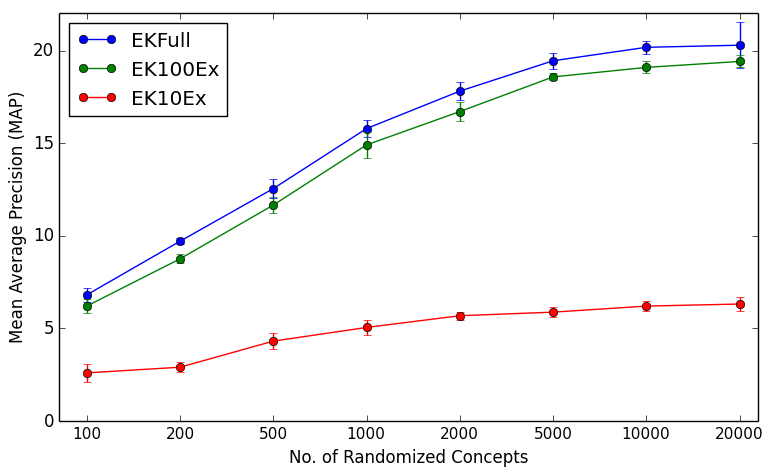
\includegraphics[width=1\textwidth]{images/p_exp2.png}}
    (a) On the MED 2012 KINDREDTEST dataset
  \end{column}

  \begin{column}{0.5\textwidth}
    \centerline{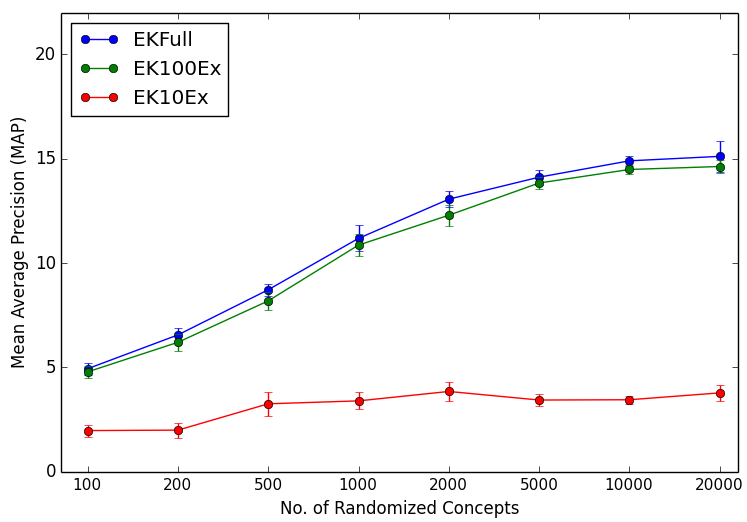
\includegraphics[width=1\textwidth]{images/p_exp2_mt.png}}
    (b) On the MED 2012 MEDTEST dataset
  \end{column}
\end{columns}
\bigskip
 
The best performance can be obtained using around ten thousands of totally random labeled concept detectors!
  
\end{frame}

\begin{frame}[t]{Influence of Number of Pseudo Positives?}
\bigskip

\begin{columns}
  \begin{column}{0.5\textwidth}
    \centerline{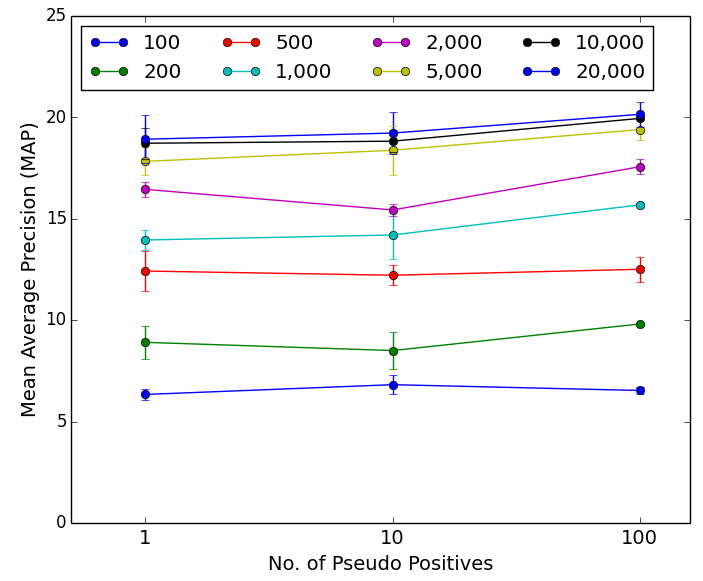
\includegraphics[width=1\textwidth]{images/p_exp3.png}}
    (a) On the MED 2012 KINDREDTEST dataset
  \end{column}

  \begin{column}{0.5\textwidth}
    \centerline{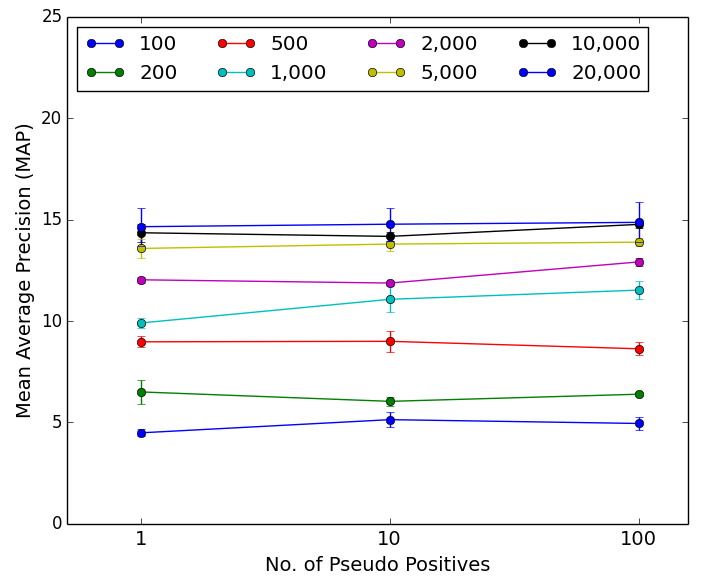
\includegraphics[width=1\textwidth]{images/p_exp3_mt.png}}
    (b) On the MED 2012 MEDTEST dataset
  \end{column}
\end{columns}
\bigskip

The detection performance does not depend on the number of pseudo positives!

\end{frame}
% % part 5

\begin{frame}[t]{Issues}
\begin{itemize}
\item Can we identify key video segments? 
\item How about classes of video segments? Can be a set of generic classes (generic sub events), or depending of each event (sub events specific to each event)?
\item How to combine the analysis results of video segment?
\item How to adapt to ad hoc case?
\begin{itemize}
\item key video segments should be automatically detected
\item generic set of sub events should be pre-defined
\item or sub events should be adaptively generated from given event kit
\end{itemize}

\end{itemize}
\end{frame}

\end{document}